\documentclass[tikz,border=2pt]{standalone}
\usepackage{amsmath,amssymb}
% sans serif for text and math
\renewcommand{\familydefault}{\sfdefault}
\usepackage[eulergreek]{sansmath}
\sansmath
\usepackage{pgfplots}
\pgfplotsset{compat=1.18}
\usetikzlibrary{arrows.meta}
% match the R figures in estimation.qmd
\definecolor{ctrl}{HTML}{1E90FF}  % dodgerblue
\definecolor{trt}{HTML}{FF6A6A}   % indianred1

\begin{document}
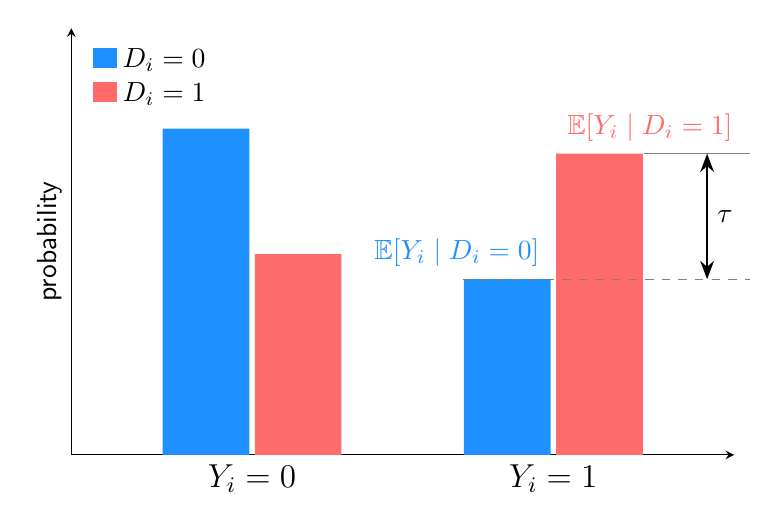
\begin{tikzpicture}
  % P(Y_i = 1 | D_i = d) = E[Y_i | D_i = d]
  \def\pzero{0.35}
  \def\pone{0.6}
  \pgfmathsetmacro{\qzero}{1-\pzero}
  \pgfmathsetmacro{\qone}{1-\pone}
  \begin{axis}[
      width=10cm, height=7cm,
      ybar, bar width=1.1cm,
      axis lines=left,
      ymin=0, ymax=0.85,
      xmin=-0.6, xmax=1.6,
      major tick length=0pt,
      xtick={0,1}, xticklabels={$Y_i = 0$, $Y_i = 1$},
      ytick=\empty, ylabel={probability},
      x tick label style={font=\large},
      legend style={draw=none, at={(0.02,0.98)}, anchor=north west},
      legend image code/.code={\fill[#1] (0cm,-0.1cm) rectangle (0.3cm,0.15cm);},
      clip=false,
    ]
    \addplot[draw=none, fill=ctrl] coordinates {(0,\qzero) (1,\pzero)};
    \addplot[draw=none, fill=trt] coordinates {(0,\qone) (1,\pone)};
    \legend{$D_i = 0$, $D_i = 1$}

    % bar centers for Y = 1 (ybar shifts each series by half a bar + gap)
    \coordinate (c1) at ([xshift=-0.55cm-1.5pt]axis cs:1,\pzero);
    \coordinate (t1) at ([xshift=0.55cm+1.5pt]axis cs:1,\pone);

    % mean labels
    \node[ctrl, above=1pt, align=center, anchor=south east]
      at ([xshift=0.55cm]c1) {$\mathbb{E}[Y_i \mid D_i = 0]$};
    \node[trt, above=1pt, align=center, anchor=south west]
      at ([xshift=-0.55cm]t1) {$\mathbb{E}[Y_i \mid D_i = 1]$};

    % tau: vertical gap between the Y = 1 bars
    \draw[thin, dashed, gray] ([xshift=-0.55cm]c1) -- ([xshift=1.9cm]c1 -| t1);
    \draw[{Stealth}-{Stealth}, thick]
      ([xshift=1.35cm]c1 -| t1) -- node[right] {$\tau$} ([xshift=1.35cm]t1);
    \draw[thin, gray] ([xshift=0.55cm]t1) -- ([xshift=1.9cm]t1);
  \end{axis}
\end{tikzpicture}
\end{document}
